\chapter{F-15C Parameter Extraction Data}
\renewcommand\thesection{\Alpha {A}}

\label{section:dragpolar}
\label{app: polar}
\begin{verbatim}
0F-15C                               
 GUN                                      
0POLAR DRAG OUTPUT
\end{verbatim}
\begin{figure}[H]
    \centering
    
\includegraphics[width = 15cm]{Thesis/Appendices/Drag_Polar_Example.png}
    %\caption{}
    %\label{fig:my_label}
\end{figure}

\chapter{Tradeoff Comparisons}
\label{app:tradeoffComps}
\begin{figure}[H]%
    \centering
    \subfloat[Comparison at 30,000 ft]{{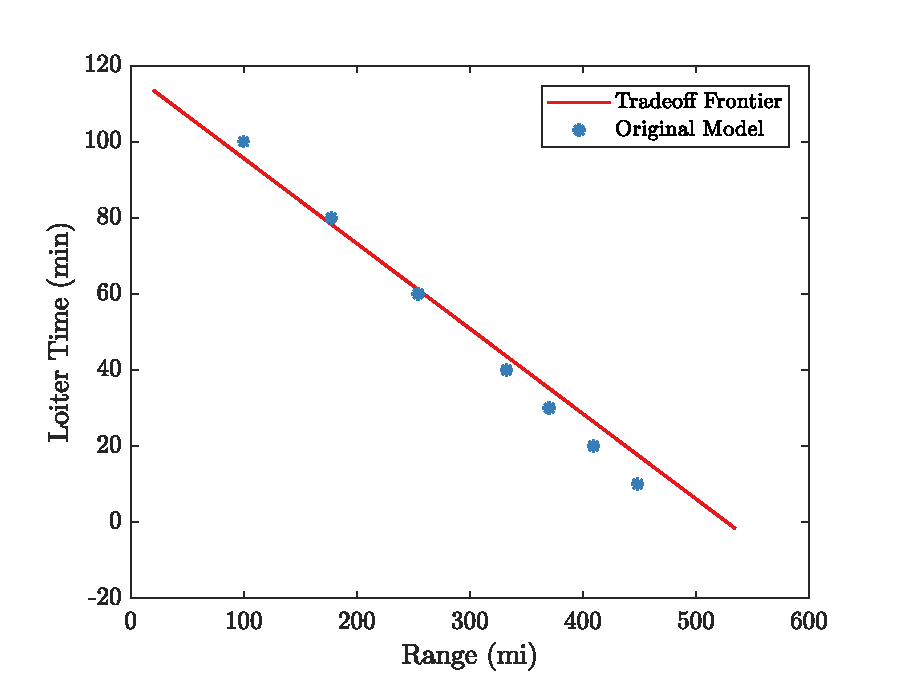
\includegraphics[width=5cm]{Thesis/Analysis/Tradeoff_Pics/30000f16.eps} }}%
    \qquad
    \subfloat[Comparison at 20,000 ft]{{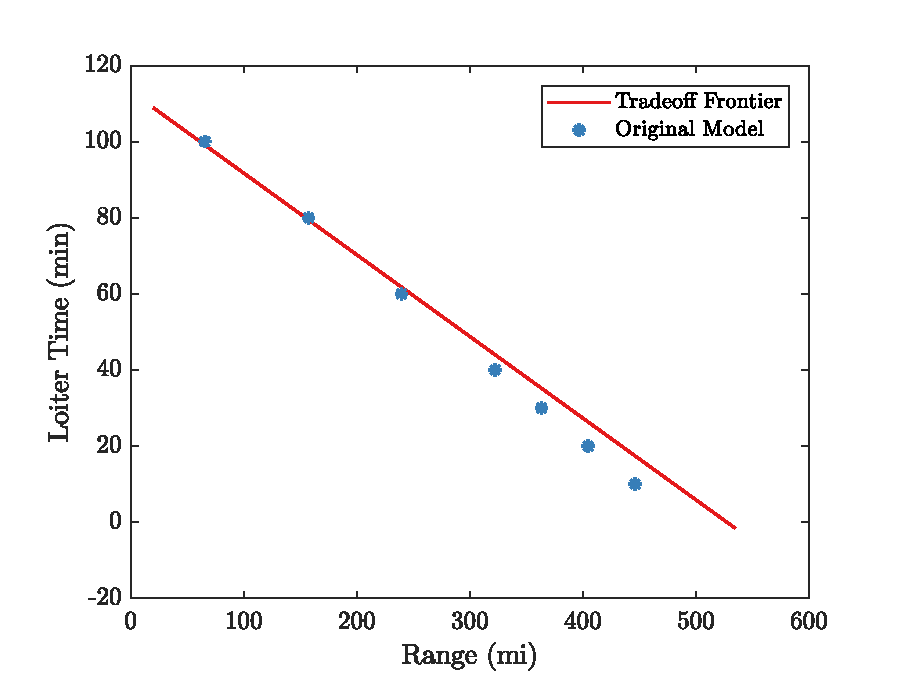
\includegraphics[width=5cm]{Thesis/Analysis/Tradeoff_Pics/20000f16.eps} }}%
    \qquad
    \subfloat[Comparison at 10,000 ft]{{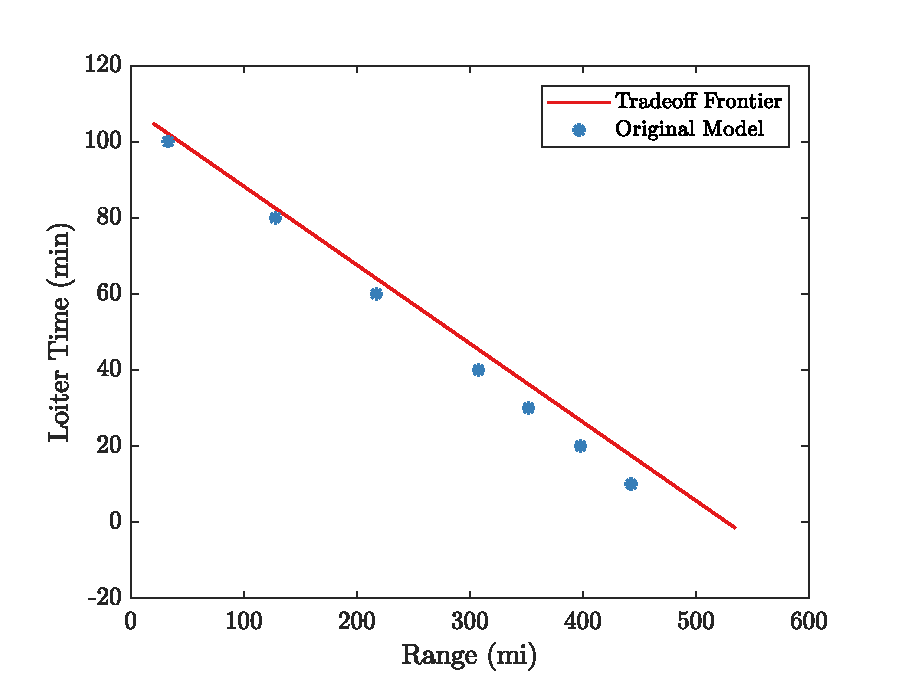
\includegraphics[width = 5cm]{Thesis/Analysis/Tradeoff_Pics/10000f16.eps} }}
    \caption{Tradeoff Comparison for F-16C}%
    \label{fig:tradef16}
\end{figure}

\begin{figure}[H]%
    \centering
    \subfloat[Comparison at 30,000 ft]{{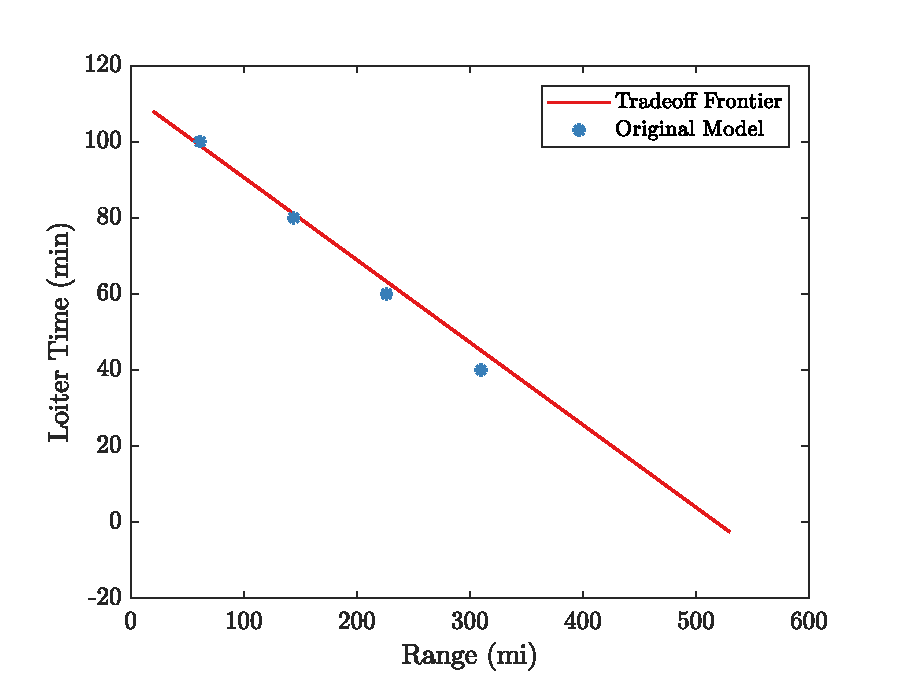
\includegraphics[width=5cm]{Thesis/Analysis/Tradeoff_Pics/30000c1.eps} }}%
    \qquad
    \subfloat[Comparison at 20,000 ft]{{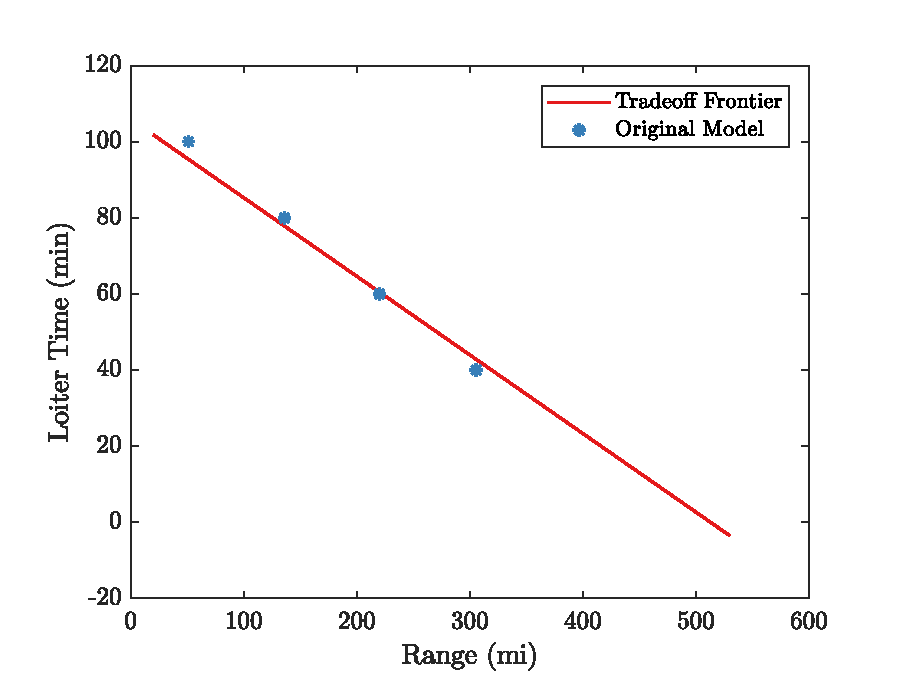
\includegraphics[width=5cm]{Thesis/Analysis/Tradeoff_Pics/20000c1.eps} }}%
    \qquad
    \subfloat[Comparison at 10,000 ft]{{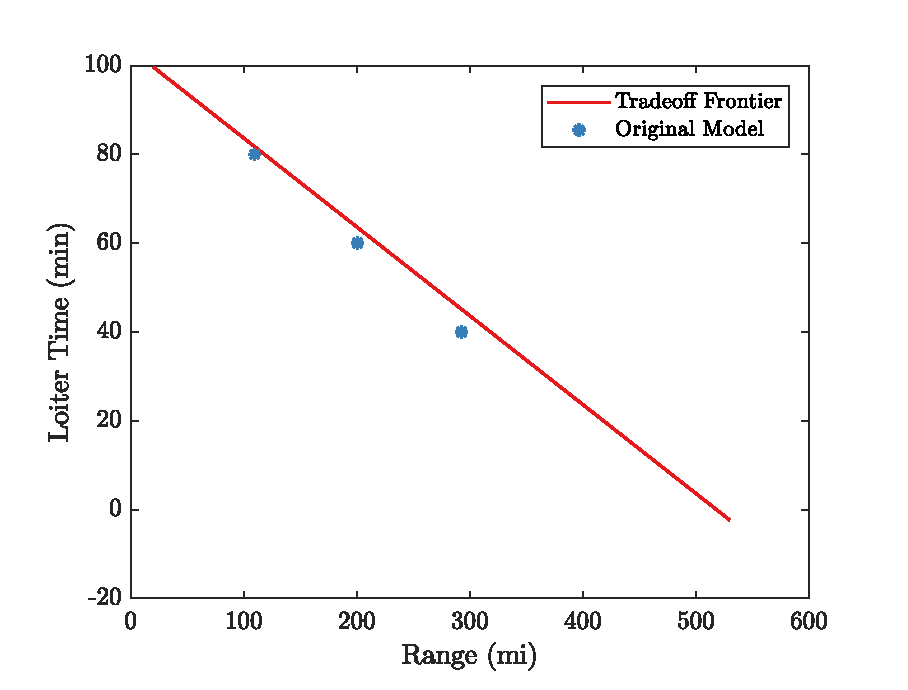
\includegraphics[width = 5cm]{Thesis/Analysis/Tradeoff_Pics/10000c1.eps} }}
    \caption{Tradeoff Comparison for AC1-000}%
    \label{fig:tradec1}
\end{figure}

\begin{figure}[H]%
    \centering
    \subfloat[Comparison at 30,000 ft]{{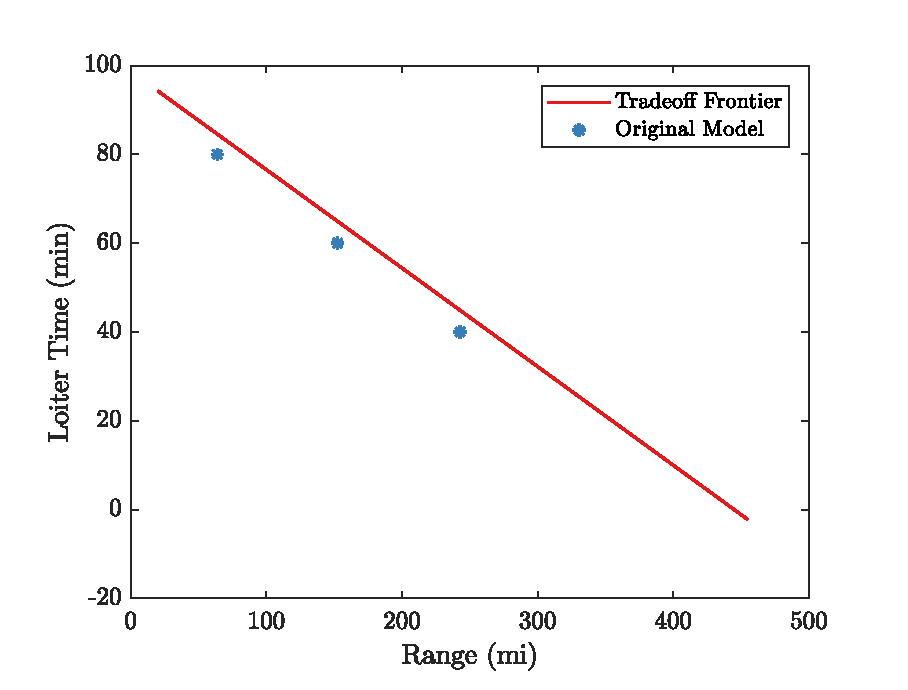
\includegraphics[width=5cm]{Thesis/Analysis/Tradeoff_Pics/30000c2.eps} }}%
    \qquad
    \subfloat[Comparison at 20,000 ft]{{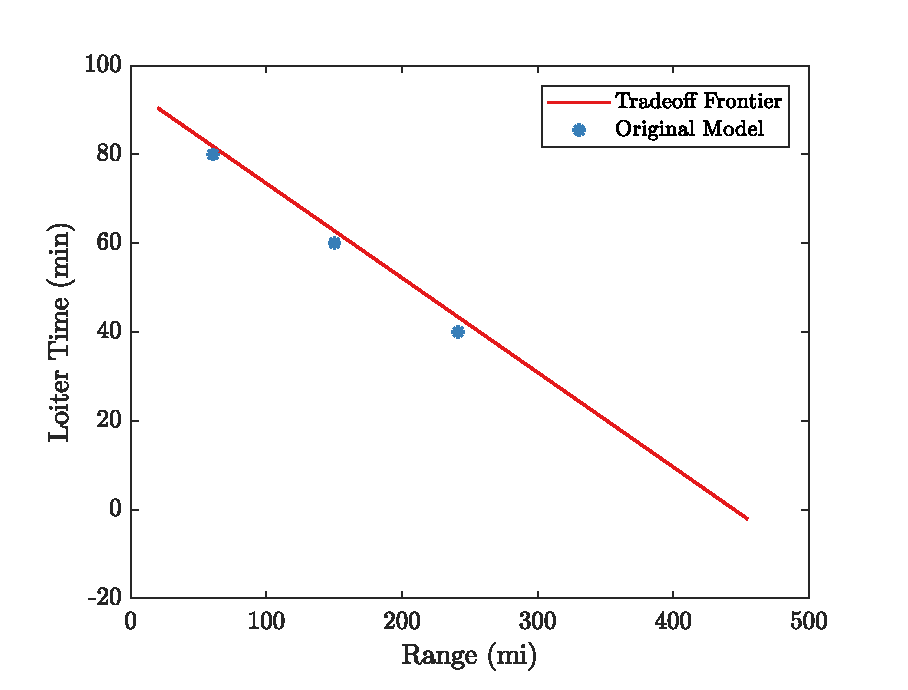
\includegraphics[width=5cm]{Thesis/Analysis/Tradeoff_Pics/20000c2.eps} }}%
    \qquad
    \subfloat[Comparison at 10,000 ft]{{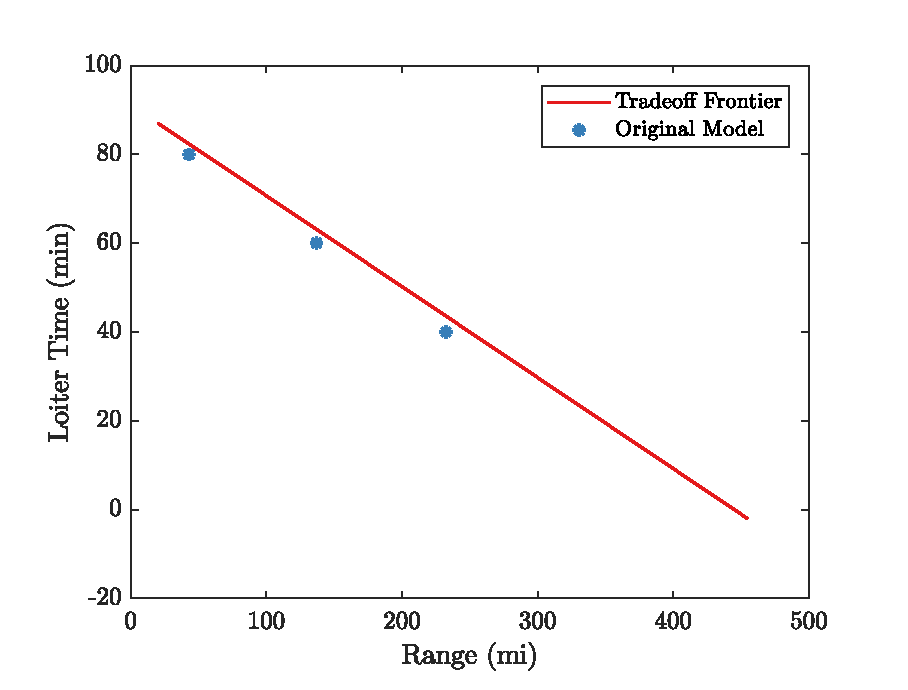
\includegraphics[width = 5cm]{Thesis/Analysis/Tradeoff_Pics/10000c2.eps} }}
    \caption{Tradeoff Comparison for AC2-000}%
    \label{fig:tradec2}
\end{figure}

\begin{figure}[H]%
    \centering
    \subfloat[Comparison at 30,000 ft]{{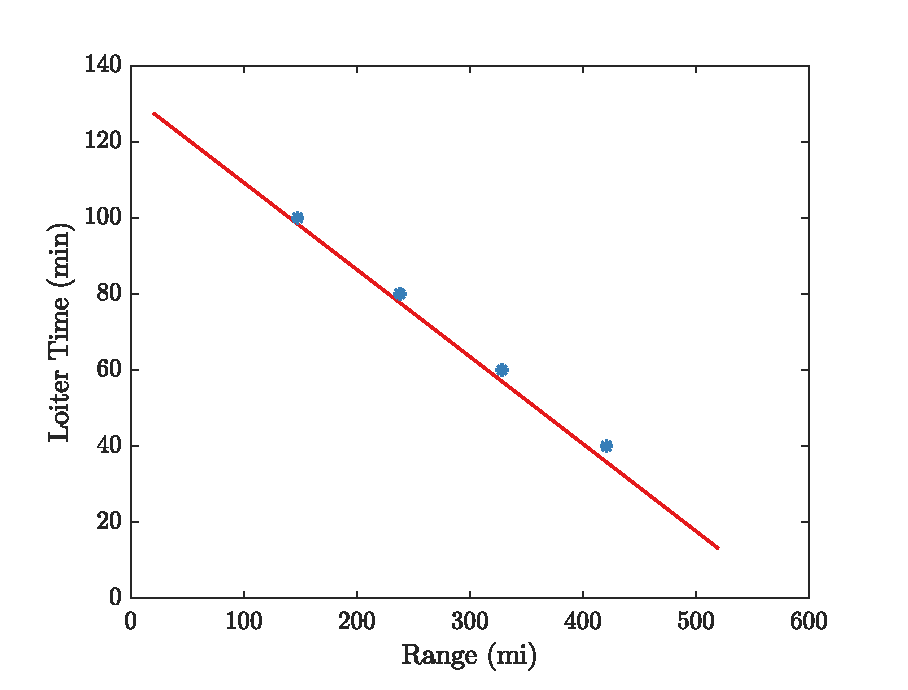
\includegraphics[width=5cm]{Thesis/Analysis/Tradeoff_Pics/30000c3.eps} }}%
    \qquad
    \subfloat[Comparison at 20,000 ft]{{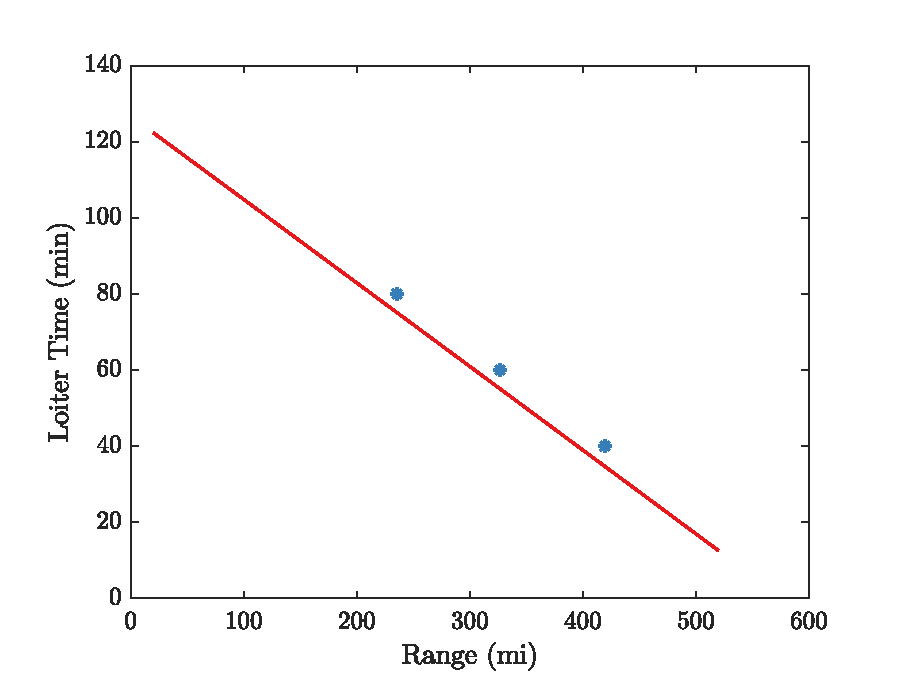
\includegraphics[width=5cm]{Thesis/Analysis/Tradeoff_Pics/20000c3.eps} }}%
    \qquad
    \subfloat[Comparison at 10,000 ft]{{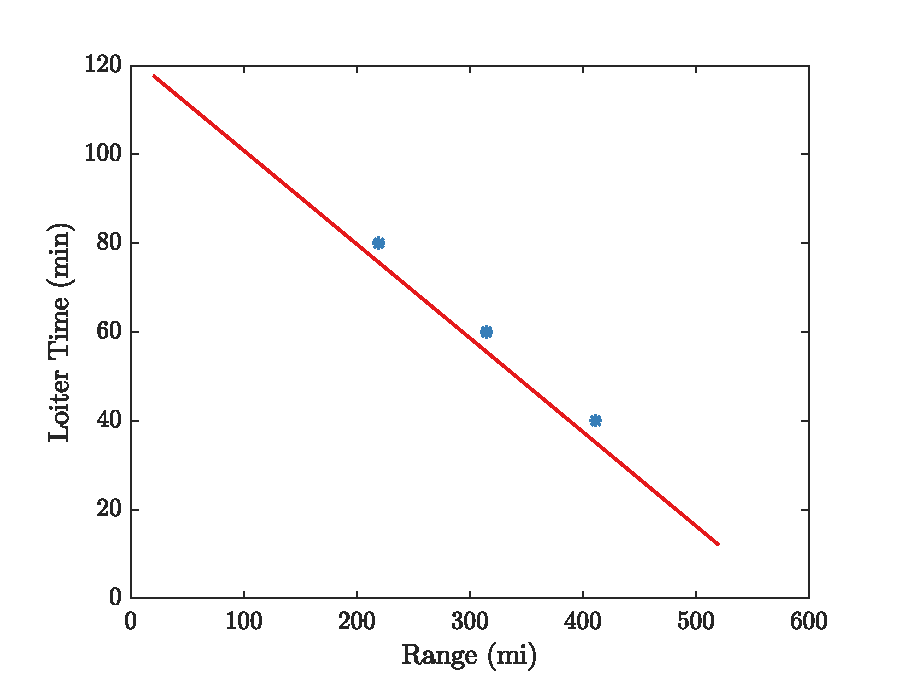
\includegraphics[width = 5cm]{Thesis/Analysis/Tradeoff_Pics/10000c3.eps} }}
    \caption{Tradeoff Comparison for AC3-000}%
    \label{fig:tradec3}
\end{figure}

\begin{figure}[H]%
    \centering
    \subfloat[Comparison at 30,000 ft]{{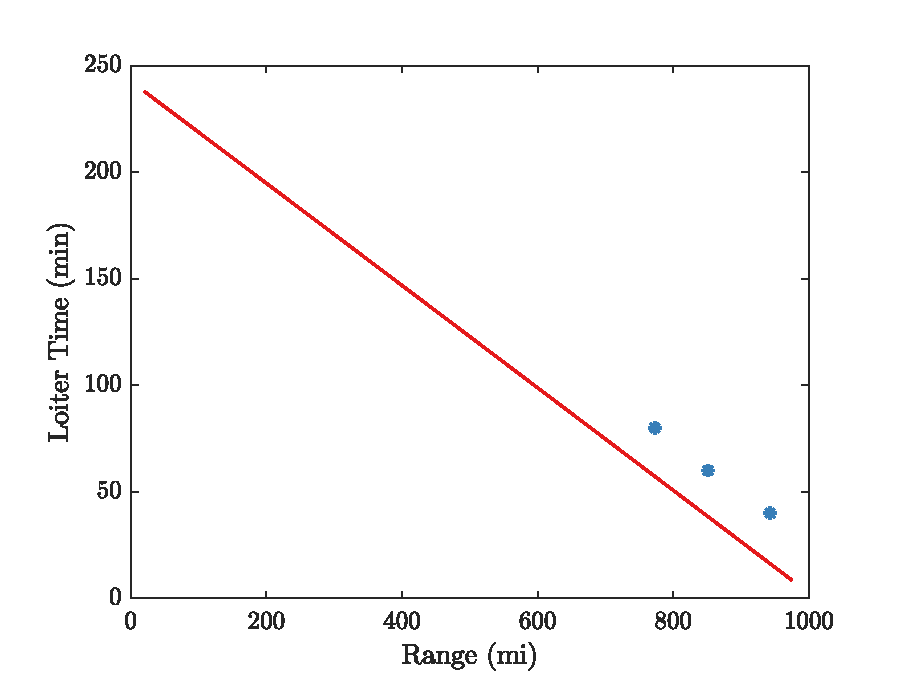
\includegraphics[width=5cm]{Thesis/Analysis/Tradeoff_Pics/30000c4.eps} }}%
    \qquad
    \subfloat[Comparison at 20,000 ft]{{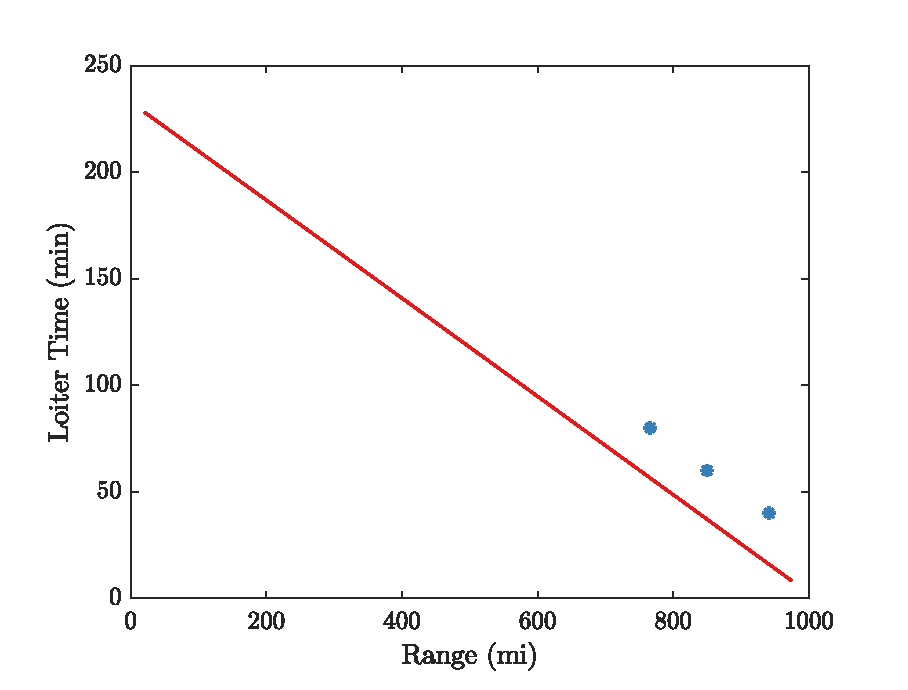
\includegraphics[width=5cm]{Thesis/Analysis/Tradeoff_Pics/20000c4.eps} }}%
    \qquad
    \subfloat[Comparison at 10,000 ft]{{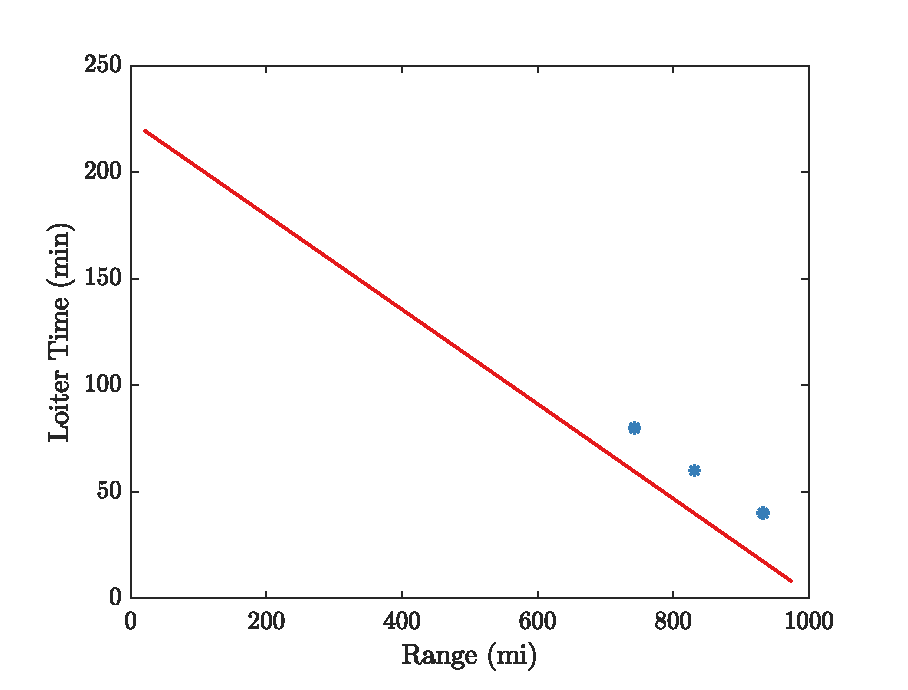
\includegraphics[width = 5cm]{Thesis/Analysis/Tradeoff_Pics/10000c4.eps} }}
    \caption{Tradeoff Comparison for AC4-000}%
    \label{fig:tradec4}
\end{figure}

\chapter{MATLAB Code for Structure Tradeoffs}
\renewcommand\thesection{\Alpha {A}}
\section{Linear Tradeoff Code}
\lstinputlisting[language = MATLAB]{Thesis/Appendices/Code/simpleplan.m}
\renewcommand\thesection{\Alpha {B}}
\section{Nonlinear Tradeoff Code}
\lstinputlisting[language = MATLAB]{Thesis/Appendices/Code/FixForWeight.m}
\renewcommand\thesection{\Alpha {C}}
\section{Example Structure Code}
\lstinputlisting[language = MATLAB]{Thesis/Appendices/Code/StructForNL_F15.m}

\chapter{MATLAB Code for Optimization Formulations}
\renewcommand\thesection{\Alpha {A}}
\section{Assignment Problem}
\lstinputlisting[language = MATLAB]{Thesis/Appendices/Code/AssignmentProblemTry.m}

\renewcommand\thesection{\Alpha {B}}
\section{Random Priority Assignment Problem}
\lstinputlisting[language = MATLAB]{Thesis/Appendices/Code/RandPriorityAssignment.m}

\renewcommand\thesection{\Alpha {C}}
\section{Random Priority Assignment Problem with Multiple Structures}
\lstinputlisting[language = MATLAB]{Thesis/Appendices/Code/DiffStructuresAssignmentProblem.m}

\renewcommand\thesection{\Alpha {D}}
\section{Decision Dependent Formulation}
\lstinputlisting[language = MATLAB]{Thesis/Appendices/Code/LargerDecisionDependentFormulation.m}

\renewcommand\thesection{\Alpha {E}}
\section{Decision Dependent Formulation with Constrained Loiter Fuel}
\lstinputlisting[language = MATLAB]{Thesis/Appendices/Code/ExtraConstrainedForEnduranceDDF.m}

\chapter{Python Class Method}
\renewcommand\thesection{\Alpha {A}}
\section{Aircraft Class Structure}
\lstinputlisting[language = Python]{Thesis/Appendices/Code/AircraftClass.py}

\renewcommand\thesection{\Alpha {B}}
\section{Radius and Distance Method}
\lstinputlisting[language = Python]{Thesis/Appendices/Code/RadiusCode.py}

\renewcommand\thesection{\Alpha {C}}
\section{Model Inputs Text Parser}
\lstinputlisting[language = Python]{Thesis/Appendices/Code/modelinputs.py}

\renewcommand\thesection{\Alpha {D}}
\section{Example Usage}
\lstinputlisting[language = Python]{Thesis/Appendices/Code/exampleusage.py}